\section{Exponential growth and decay}

It is 2:00 a.m.\ and Joe is up studying.  The dorm has quieted down, but Joe's feeling mighty jittery.  He  drank 5 large mugs of coffee in the past few hours and all that caffeine is peaking in his system now.  At around 200 mg per mug, Joe wonders when his caffeine levels will drop down to where he can sleep a little.  

First things first:  staying up that late to study is probably a bad idea.  I mean, who can think properly at 2:00 in the morning?  And, how tired is Joe going to be by the time his test rolls around?  Plus, we know that
$$5 \text{ mugs} \ast \frac{200 \text{ mg}}{\text{mug}} = 5 \times 200 = \text{1,000 mg}$$
which is a lot of caffeine, probably more than he needed to stay awake.  

At this point Joe is stuck so let's help him. Let's say that at 2:00 a.m.\ he has \text{1,000} mg of caffeine in his blood.  Joe searches online and discovers that 13\% of the caffeine should leave his body each hour and below 300 mg he should be fine.  When will that happen?

We know how percent increase works, but here the caffiene is leaving his body according to a percent decrease.  I guess we need to figure it out one step at a time.  After one hour (by 3:00 a.m.), Joe will have 
$$  \text{1,000} \text{ mg} - 13 \% \text{ of }  \text{1,000} \text{ mg} =  \text{1,000}- .13 \times  \text{1,000} =  \text{1,000} - 130 = 870 \text{ mg}$$
By 4:00 a.m.\ (after 2 hours), Joe will have
$$ 870 \text{ mg} - 13 \% \text{ of } 870 \text{ mg} = 870 - .13 \times 870 = 870 - 113.1 =  756.9 \text{ mg}$$

Wait a minute.  When we calculated 13\% decrease on  \text{1,000} mg we got 870 mg.  That's 87\% of \text{1,000}.  Yeah, that's right, take off 13\% and you should be left with 87\% of what you started with because $100\% - 13\% = 87\%$.
So we could have calculated 
$$ .87 \times \text{1,000} = 870 \text{ mg}$$
and then $$.87 \times 870 = 756.9 \text{ mg}$$
Aha, to find the amount after a 13\% decrease we just multiply by .87.

Still nowhere near 300 mg so fast-forward.  For example, after 5 hours (at 7:00 a.m.), we need to multiply  \text{1,000} by .87 five times
$$1000 \ast .87 \ast .87 \ast .87 \ast .87 \ast .87=  \text{1,000} \ast .87^5$$
where we use a power to abbreviate repeatedly multiplying.  So
$$1000 \ast .87^5 =  \text{1,000} \times .87 \wedge 5 = 498.420920\ldots \approx 498.4 \text{ mg}$$

The bad news is that it's 7:00 a.m.\ and Joe is still too jittery to sleep. 
The good news is that we can write the equation.  The variables are 
\begin{center}
\begin{tabular} {l} 
$J=$ Joe's caffeine level (mg) $\sim$ dep \\ 
$H =$ time (hours since 2:00 a.m.) $\sim$ indep \\
\end{tabular}
\end{center}
Our equaton must be $$ J = \text{1,000} \ast.87^H$$
Notice this equation fits our template for an exponential equation.
$$\text{dep }=\text{ start } \ast \text{growth factor}^{\text{indep}}$$

A little terminology here. When a function is exponential but decreasing, it's called \textbf{exponential decay}.  It sounds a little odd to say ``growth factor'' if the quantity is getting smaller so we sometimes say \textbf{decay factor} instead.   We know from the \textsc{Percent Change Formula} that the growth factor ($g$) can be found from the growth rate (r) by the formula $g=1+r$.  If we think of 13\% decrease as negative growth rate, $r=-13\%=-.13$, then the formula still works to find the decay factor ($g$)
$$g= 1 + r = 1 + -.13 = 1-.13 = .87$$  

Back to jittery Joe.  Let's summarize what we've found and add a few more times to see when Joe's caffeine level should fall below 300 mg.  
\begin{center}
\begin{tabular} {|c| |c |c |c |c |c |c |c |c |c |c|}\hline
time & 2:00 & 3:00  & 4:00 & 5:00  & 6:00  & 7:00 & 8:00 & 9:00 & 10:00 & 11:00 \\ \hline
$H$ & 0 & 1 & 2 & 3 & 4 & 5 & 6 & 7 & 8 & 9\\ \hline
$J$ & \text{1,000} & 870 & 756.9 & 658.5 & 572.9 & 498.4 & 433.6 & 377.3 & 328.2 & 285.5 \\ \hline
vs.\ 300 & high & high& high& high& high& high& high& high& high& low\\ \hline
\end{tabular}
\end{center}
That means Joe should be able to fall asleep by around 11:00 a.m.  Exactly when his exam starts.  Sorry, Joe.

We could have solved the equation instead.  We were looking for $J = 300$.  Using our equation $J = \text{1,000} \ast .87^H$ we get
$$ \text{1,000} \ast .87^H=300$$
Divide each side \text{1,000} to get
$$ \frac{\cancel{\text{1,000}} \ast .87^H}{\cancel{\text{1,000}}}= \frac{300}{\text{1,000}}$$
which simplifies to $$.87^H = \frac{300}{\text{1,000}} = 300 \div \text{1,000} = .3$$

We find ourselves in the familiar situation -- solving to find the exponent.  Logs to the rescue.  By the
\textsc{The Log-Divides Formula} with growth factor $g=.87$ and value $v= .3$ we get $$Y =  \frac{\log (v)}{\log(g)}=  \frac{\log (.3)}{\log(.87)} =  \log (.3) \div \log (.87) =  8.64537506\ldots \approx 9 $$ 
which corresponds to 11:00 a.m.  Same answer.  Much quicker.

Quick side note.  We could have rounded to 8.64 hours and then converted units to get
$$.64 \text{ hours} \ast \frac{60 \text{ minutes}}{1 \text{ hour}} = .64 \times 60 = 38.4 \approx 39 \text{ minutes}$$
Counting from  2:00 a.m., we see that Joe's caffeine levels drop below 300 mg at 10:39 a.m.  Since we are approximating throughout the problem, we should round to 11:00 a.m.\  anyway.

Let's calculate the rate of change and think about what it means.  During the first hour,
$$\text{rate of change} =  \frac{\text{change dep}}{\text{change indep}} 
= \frac{870-\text{1,000 mg}}{\text{3:00 a.m.} - \text{2:00 a.m.}} = \frac{-130 \text{ mg}}{1 \text{ hour}} = -130 \text{ mg/hour}$$
Was the rate of change supposed to be negative? Sure.  Joe's caffeine level is dropping.  Any decreasing function has a negative rate of change.
And, as exam approaches,
$$\text{rate of change} =  \frac{\text{change dep}}{\text{change indep}}  = \frac{285.5-328.2 \text{ mg}}{\text{11:00 a.m.} - \text{10:00 a.m.}} = \frac{-42.7 \text{ mg}}{1 \text{ hour}} \approx -43 \text{ mg/hour}$$
Joe's caffeine level was dropping faster at first and is not dropping as fast now.  

A glance at the graph confirms our findings.
 \begin{center}
\scalebox {.8} {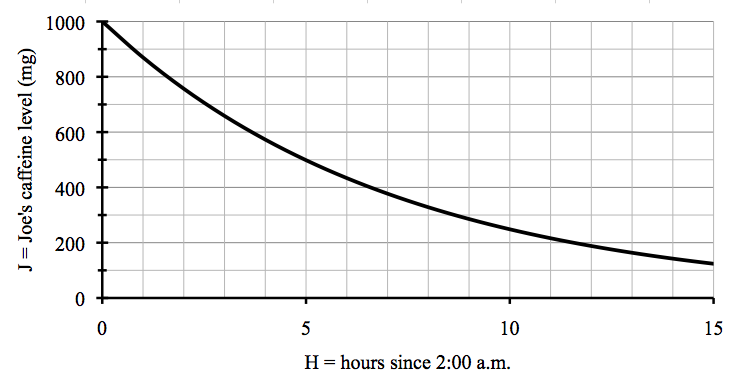
\includegraphics [width = 6in] {caffeine.png}}
\end{center}

One last thing.  There's another way to describe the decrease here.  When our story began Joe's caffeine level was around \text{1,000} mg and after 5 hours is was at 498.4 mg.  That's just about 500 mg, or half of what he started with.  We say the \textbf{half-life} of caffeine is around 5 hours.  

Doesn't sound very important but check this out.  Start with \text{1,000} mg.  After 5 hours, there's 500 mg left.  (Okay, approximately.)  Now go another 5 hours, which means 10 hours total.  Evaluate our equation $J = \text{1,000} \ast .87^H$ when $H =10$ to get
 $$ J = \text{1,000} \ast .87^{10} = \text{1,000} \ast .87 \wedge \underline{10} = 248.423414\ldots \approx 250$$ 
That means half of what was left is now gone.  Go another 5 hours. Lose another half. Check for yourself:
$$ J = \text{1,000} \ast .87^{15} = \text{1,000} \ast .87 \wedge \underline{15} = 123.819426\ldots \approx 125$$ 
And so on.  Cool.

%\newpage

%%\section{Exponential growth and decay}

 \begin{center}
\line(1,0){300} %\line(1,0){250}
\end{center}

\section*{Homework}

\noindent \textbf{Start by doing Practice exercises \#1-4 in the workbook.}

\bigskip

\noindent \textbf{Do you know \ldots}

\begin{itemize}
\item How to write an exponential equation given the starting amount and percent decrease? 
\item What ``half-life'' means? 
\item What ``doubling time'' means?     
\item What the graph of exponential growth and exponential decay look like? 
\item Why the rate of change for exponential decay is negative? 
 \item[~] \textbf{If you're not sure, work the rest of exercises and then return to these questions.  Or, ask your instructor or a classmate for help.} 
\end{itemize}

\subsection*{Exercises}

\begin{enumerate} 
\setcounter{enumi}{4}
\item Joe's girlfriend Ceyda starts the day by downing two cans of Red Bull, containing a total of 160 mg of caffeine.  Her body eliminates the caffeine at a slightly slower rate of 12\% each hour.  
\begin{enumerate}
\item Name the variables and write an equation to model this situation.  
\item What's the half-life of caffeine for Ceyda?  Set up and solve an equation.
\item Ceyda heard that drinking a glass of water an hour can help eliminate caffeine faster.  If so, would the half-life be shorter or longer?  Explain.
\end{enumerate}

\item  The population of bacteria in a culture dish begins at 2,000 and will triple every day.  
\begin{enumerate}
\item Name the variables, including units and dependence.
\item Make a table showing the number of bacteria at the start and after 1 day, 2 days, and 3 days.
\item Write an equation illustrating bacterial growth.
\item Your equation should fit the template for an exponential equation. What is the daily growth factor?
\item Use your equation to extend your table to include 10 days, 20 days, and 30 days. Be careful to report the large numbers appropriately.  \emph{Hint: scientific notation}
\item The dish can support around 1 million bacteria.  When does that happen?  Give your answer to the nearest hour.
\item Draw a graph, including a table of reasonable values.  Remember, the dish can only support up to 1 million bacteria, so your graph should go up to 1 million.
\end{enumerate}

\item Tenzin bought a house for \$291,900 but the housing market collapsed and his house value dropped 4.1\% each year. 
 \begin{enumerate}
\item Name the variables and write an equation relating them.
\item At this rate, how many years would it take for the value of Tenzin's house to drop below \$240,000?  Use successive approximation to guess the year.
\item Now set up and solve an equation.
\end{enumerate}

\item One modern technique for cleaning waste water involves the use of constructed (man-made) wetlands.  Wetlands act as a natural biofilter for various contaminants in the waste water. After each month in the wetlands, only about \nicefrac{1}{4} of the contaminants remain in any given sample.  Suppose a sample had 8 grams of contaminants before processed in the constructed wetlands.
\begin{enumerate}
\item How much would remain in the sample after 1 month?  2 months?  3 months?
\item Name the variables and write an equation relating them.
\item Your equation should fit the template for an exponential equation. What is the monthly decay factor?
\item According to your equation, when will the contaminants fall below 1 mg?  1 $\mu$g?  Remember $1 \text{ gram} = \text{1,000 mg}$ and $1 \text{ gram} = \text{1,000,000 } \mu \text{g}$
\item Draw a graph illustrating the waste water treatment process for the first 6 months.
\end{enumerate}  % DATA is wastewater.xlsx

\item Hibbing, Minnesota is the hometown of baseball star Roger Maris, basketball great Kevin McHale, the Greyhound Bus lines, the Hull-Rust-Mahoning Open Pit Iron Mine and, perhaps most famously, the childhood home of songwriter Bob Dylan.
It is not a big town.  In 2000 the population  was reported at  17,071 residents, with an expected decrease of around 0.4\% per year.
\begin{enumerate}
\item What is the annual decay factor?
\item Name the variables and write an equation relating them.
\item Based on these estimates, what was the anticipated population of Hibbing in 2010?
\item The actual 2010 U.S.\ Census estimate of Hibbing's population was 16,361 people.  Was the decrease slower or faster than expected?  Was the decay rate more or less than 0.4\%?  Explain.
\end{enumerate}

\item Donations to a local food shelf have increased 35\% over last year.  There were 3,400 pounds of food donated last year. \hfill \emph{Story also appears in 5.3 \#4}
\begin{enumerate}
\item Name the variables, measuring time since last year.  (Yes, it's a little awkward.)
\item Write an exponential equation relating the variables, assuming the rate of increase continues.
\item How much was donated this year?  How much is expected next year?  The year after?
\item At this rate, what is the doubling time?  That means, how long would it be until twice as much is donated.  Set up and solve an equation to answer.  Report your answer to the nearest month.
\item The agency estimates that around 12,000 pounds of food is needed each year to meet the needs of the people they serve.  In how many years will donations reach that level?  (In your answer, say how many years from now.)
\end{enumerate}


\end{enumerate}